%!TEX root = paper.tex
%%%%%%%%%%%%%%%%%%%%%%%%%%%%%%%%%%%%%%%%%%%%%%%%%%%%%%%%%%%%%%%%%%%%%%%%%%%%%%%%
\section{Overview and Background}
\label{sec:background}

Before looking at the fallacies in the literature, first some fundamental gaming terms and concepts need to be introduced. At their core video games are essentially feedback-directed real-time simulators. The game reads player input, updates the game state, and renders new screen contents. This loop repeats as long as the game is running. While the three parts are interrelated, and every component provides some form of input to the next, they may still proceed at their own intrinsic paces. The \textit{tickrate} governs the frequency of game state updates, and the \textit{framerate} determines the update rate of the output image. Popular examples for the tickrates of games servers include \SI{64}{\hertz} or \SI{128}{\hertz} for \textsc{CS:GO}, \SI{20}{\hertz} for \textsc{Minecraft}, or \SI{30}{\hertz} for \textsc{Dota 2}.


%%%%%%%%%%%%%%%%%%%%%%%%%%%%%%%%%%%%%%%%%%%%%%%%%%%%%%%%%%%%%%%%%%%%%%%%%%%%%%%%
\subsection{Framerate and Lag}
\label{sec:framerate}

Motion in video data is based on the principle of \textit{apparent motion}. In order to perceive objects to be in motion in videos, consecutive images have to appear at a certain rate which is considered to be at about \SI{16.67}{\hertz} \cite{wertheimer1912experimentelle}. Below that threshold objects will appear as two distinct objects between two consecutive still images. In contrast to traditional video media that play back at fixed framerates, e.g., \SI{24}{\hertz}, are considered to be at the low end of motion perception. Stuttering is mostly concealed due to camera artifacting such as motion blur. Video games are more flexible but also much more demanding on the framerate. Video games usually target higher framerates: at \SI{30}{\hertz}, \SI{60}{\hertz}, or even \SI{120}{\hertz}, depending on the type of game. Higher framerates enable smoother camera and object movement; they also help in increasing the interactivity and reactivity as video games constantly require input on short time scales to which the game reacts and displays the feedback.

Lag is a critically important factor for almost all games, as it governs the reaction time to in-game events. But it is often described solely on the basis of the network delay in an online game, neglecting other components that contribute to the lag, including the input device, the time to sample and process the input, the game engine and server and their tickrates, frame rendering time, and ultimately the time to display the frame on the monitor. Only if all sources are factored in the complete \textit{end-to-end lag} is captured, which can be highly variable.

%While some simple actions, say opening the menu, may have a very short lag, more complex interactions, e.g., issuing command that moves the player character in the game world, may take considerable longer to complete. Therefore, each video game will have a distinct ``lag profile''.

% TODO:
% This subsection adds the player to the architectures introduced above, highlights potential QoS and QoE (or discusses why some chosing a particular QoE metric is not useful) metrics to study. At the end of this section, the reader should agree that end to end latency is a sensible starting point to study video game qos.


%%%%%%%%%%%%%%%%%%%%%%%%%%%%%%%%%%%%%%%%%%%%%%%%%%%%%%%%%%%%%%%%%%%%%%%%%%%%%%%%
\subsection{Measurement Approaches}
\label{sec:measurementapproaches}

To properly assess such metrics some approaches come to mind. Recording in software the output stream of a video game might be the simplest approach to determine video game lag and framerate. However, this does not represent the complete end-to-end lag however, as both the controller and screen output delay are missing. Examples of this approach include \cite{Chen:2011:MLC:2072298.2071991} and \cite{6670099}, which invoke the game's menu and measure the time until it is displayed. One method to fully capture the end-to-end lag is to simultaneously record both the screen and input device through external measurements. When, e.g., using a video camera the experimenter then counts the frames between pressing a button on the input device and the action appearing on the screen and calculates the lag from this.

%A 2013 paper \cite{6574660} investigates the quality of cloud gaming interactiveness (i.e., the lag) as well as image quality by employing software recording methods on the client's computer. However, this method assumes a constant delay of game actions and may not capture the actual end-to-end lag of many of real game actions, as they are typically different from and longer as the latency of displaying a menu. A 2013 paper \cite{6574660} investigates the quality of cloud gaming interactiveness (latency) as well as image quality by employing software recording methods on the client's computer.

%Can only investigate command and update messages, not tick rate directly. Evaluate rate, IAT, and bandwidth, estimate latency (though there may be no direct link between commands and updates).

% Besides simple flow-based or packet-counting network metrics, many games also allow for deeper packet-dissecting analyses, as the often rely on standardized protocols or data formats, such as Protobuf\footnote{\url{https://developers.google.com/protocol-buffers/}} or incorporate well-known third-party multiplayer-enabling libraries. %And cloud games sometimes use derivates from the RTP-family or XMPP-based(VERIFY) protocols. 
% Additionally, almost no game encrypts its time-critical messages, enabling an easy read-out. Through these means, the specific commands can be read from the network and potentially linked to their effect on the game state in the corresponding state update messages.
%, but also potentially allowing malicious actions to be taken easily.


% \begin{figure}[!t]
% 	\centering
% 	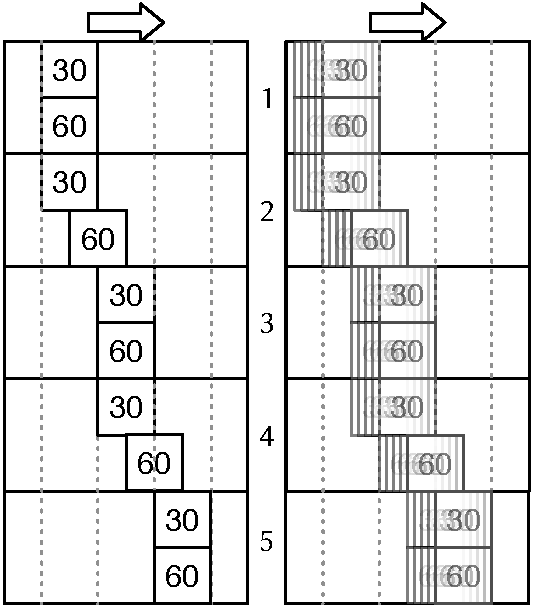
\includegraphics[width=1.0\columnwidth]{images/framerate.pdf}
% 	\caption{Effects of frame rate and motion blur on the smoothness of movement and spatial resolution. Objects move at the same speed to the right only the position os updated at different rates. A depiction of strong motion blur was added to the right-hand side.}
% \label{fig:framerate}
% \end{figure}

% The benefit of motion blur lies in its ability to conceal stutters in apparent movement due to the object and its edges being blurred, thereby reducing the positional information available on it.%, Figure~\ref{fig:framerate} illustrates this.
% Therefore, typical movie sequences usually appear to be perfectly fluid. Only for example when the camera pans at a high speed stutters in object movement or the viewport updates become apparent. Intrinsic motion blur is absent in computer generated imagery but can be artificially added to the images. While adding blur to video games can improve fluidity, it also reduces the spatial information available to the player and hampers the precision of the player's actions. Therefore it is often avoided, especially for objects in focus.

% Video games add two more factors to the frame rate consideration. The first is the issue of the monitor's refresh rate. Monitors work with a fixed, configurable image refresh rate, typically always including \SI{60}{\hertz}. If the game outputs images at an inconsistent rate or a rate lower than the monitor's refresh rate or if the framerate is not an integer multiple of the refresh rate or vice versa one of two things will happen: tearing or stuttering. % TODO: shorten and rephrase this section

% \begin{itemize}
% 	\item If the monitor fetches a frame from the graphics card's buffer while the frame is still being rendered, the result will be a mixture of the new frame in the upper half of the image and a frame which is one time interval older. This artifact is called \textbf{tearing} and should be avoided.
% 	% only the upper portion of the frame  finished, One frame split up between two refresh cycles
% 	\item Games can also be configured to postpone the rendering of a new frame until the monitor has already fetched and displayed the current frame, this is called waiting for vertical synchronization or \textbf{VSYNC}. No tearing will occur, but the \gls{IAT} of new frames might become very irregular, displaying some frames more often than others just to match the monitors refresh rate, resulting in a stuttering display. This latter stuttering effect also occurs for \SI{24}{\hertz} movies being displayed on a \SI{60}{\hertz} TV screen. Therefore most TVs additionally provide a dedicated \SI{24}{\hertz} refresh rate mode to remove the stuttering.
% \end{itemize}